\documentclass[a4paper,12pt]{article}
\usepackage[utf8]{inputenc}
\usepackage[english]{babel}
\usepackage{fancyhdr}



%Use this to customize margins
\usepackage[
  top=2cm,
  bottom=2cm,
  left=1cm,
  right=1cm,
  headheight=17pt, % as per the warning by fancyhdr
  includehead,includefoot,
  heightrounded, % to avoid spurious underfull messages
]{geometry} 

%Use this to customize headers
\pagestyle{fancy}
\fancyhf{}
\fancyhead[LE,RO]{Report version: \today}
\fancyhead[RE,LO]{ReMeltRadar 2021/22}
\fancyfoot[CE,CO]{\leftmark}
\fancyfoot[LE,RO]{\thepage}
\usepackage{graphicx}
\renewcommand{\headrulewidth}{2pt}
\renewcommand{\footrulewidth}{1pt}


\usepackage{blindtext}

%Use this to customize tables
\usepackage[table]{xcolor}
\setlength{\arrayrulewidth}{1mm}
\setlength{\tabcolsep}{18pt}
\renewcommand{\arraystretch}{1.5}
%\arrayrulecolor[HTML]{fffff}

%Use this to customize colors
\definecolor{babyblueeyes}{rgb}{0.63, 0.79, 0.95}
\definecolor{beaublue}{rgb}{0.74, 0.83, 0.9}
\definecolor{bluegray}{rgb}{0.4, 0.6, 0.8}

%Here some pre-defined commands
\newcommand{\ProtocolTable}[6]
{
\begin{table}[]
\begin{tabular}{|p{1.8cm} p{3.8cm} p{1.8cm} p{2.0cm}|}
\hline
 \rowcolor{beaublue}\textbf{Name}:&\multicolumn{3}{l}{#1} \\
 \rowcolor{beaublue}\textbf{Folder:}&\multicolumn{3}{l}{#2} \\
 \rowcolor{beaublue}\textbf{Instrument:}&#3&\textbf{Date:}&#4 \\
  \rowcolor{beaublue}\textbf{Operator:}&#5&\textbf{Location:}&#6\\
\hline
\end{tabular}
\end{table}
}

%Start the document here.

\begin{document}
\section{Summary of ReMeltRadar 2021/22}
\textbf{RD}

\begin{figure}
  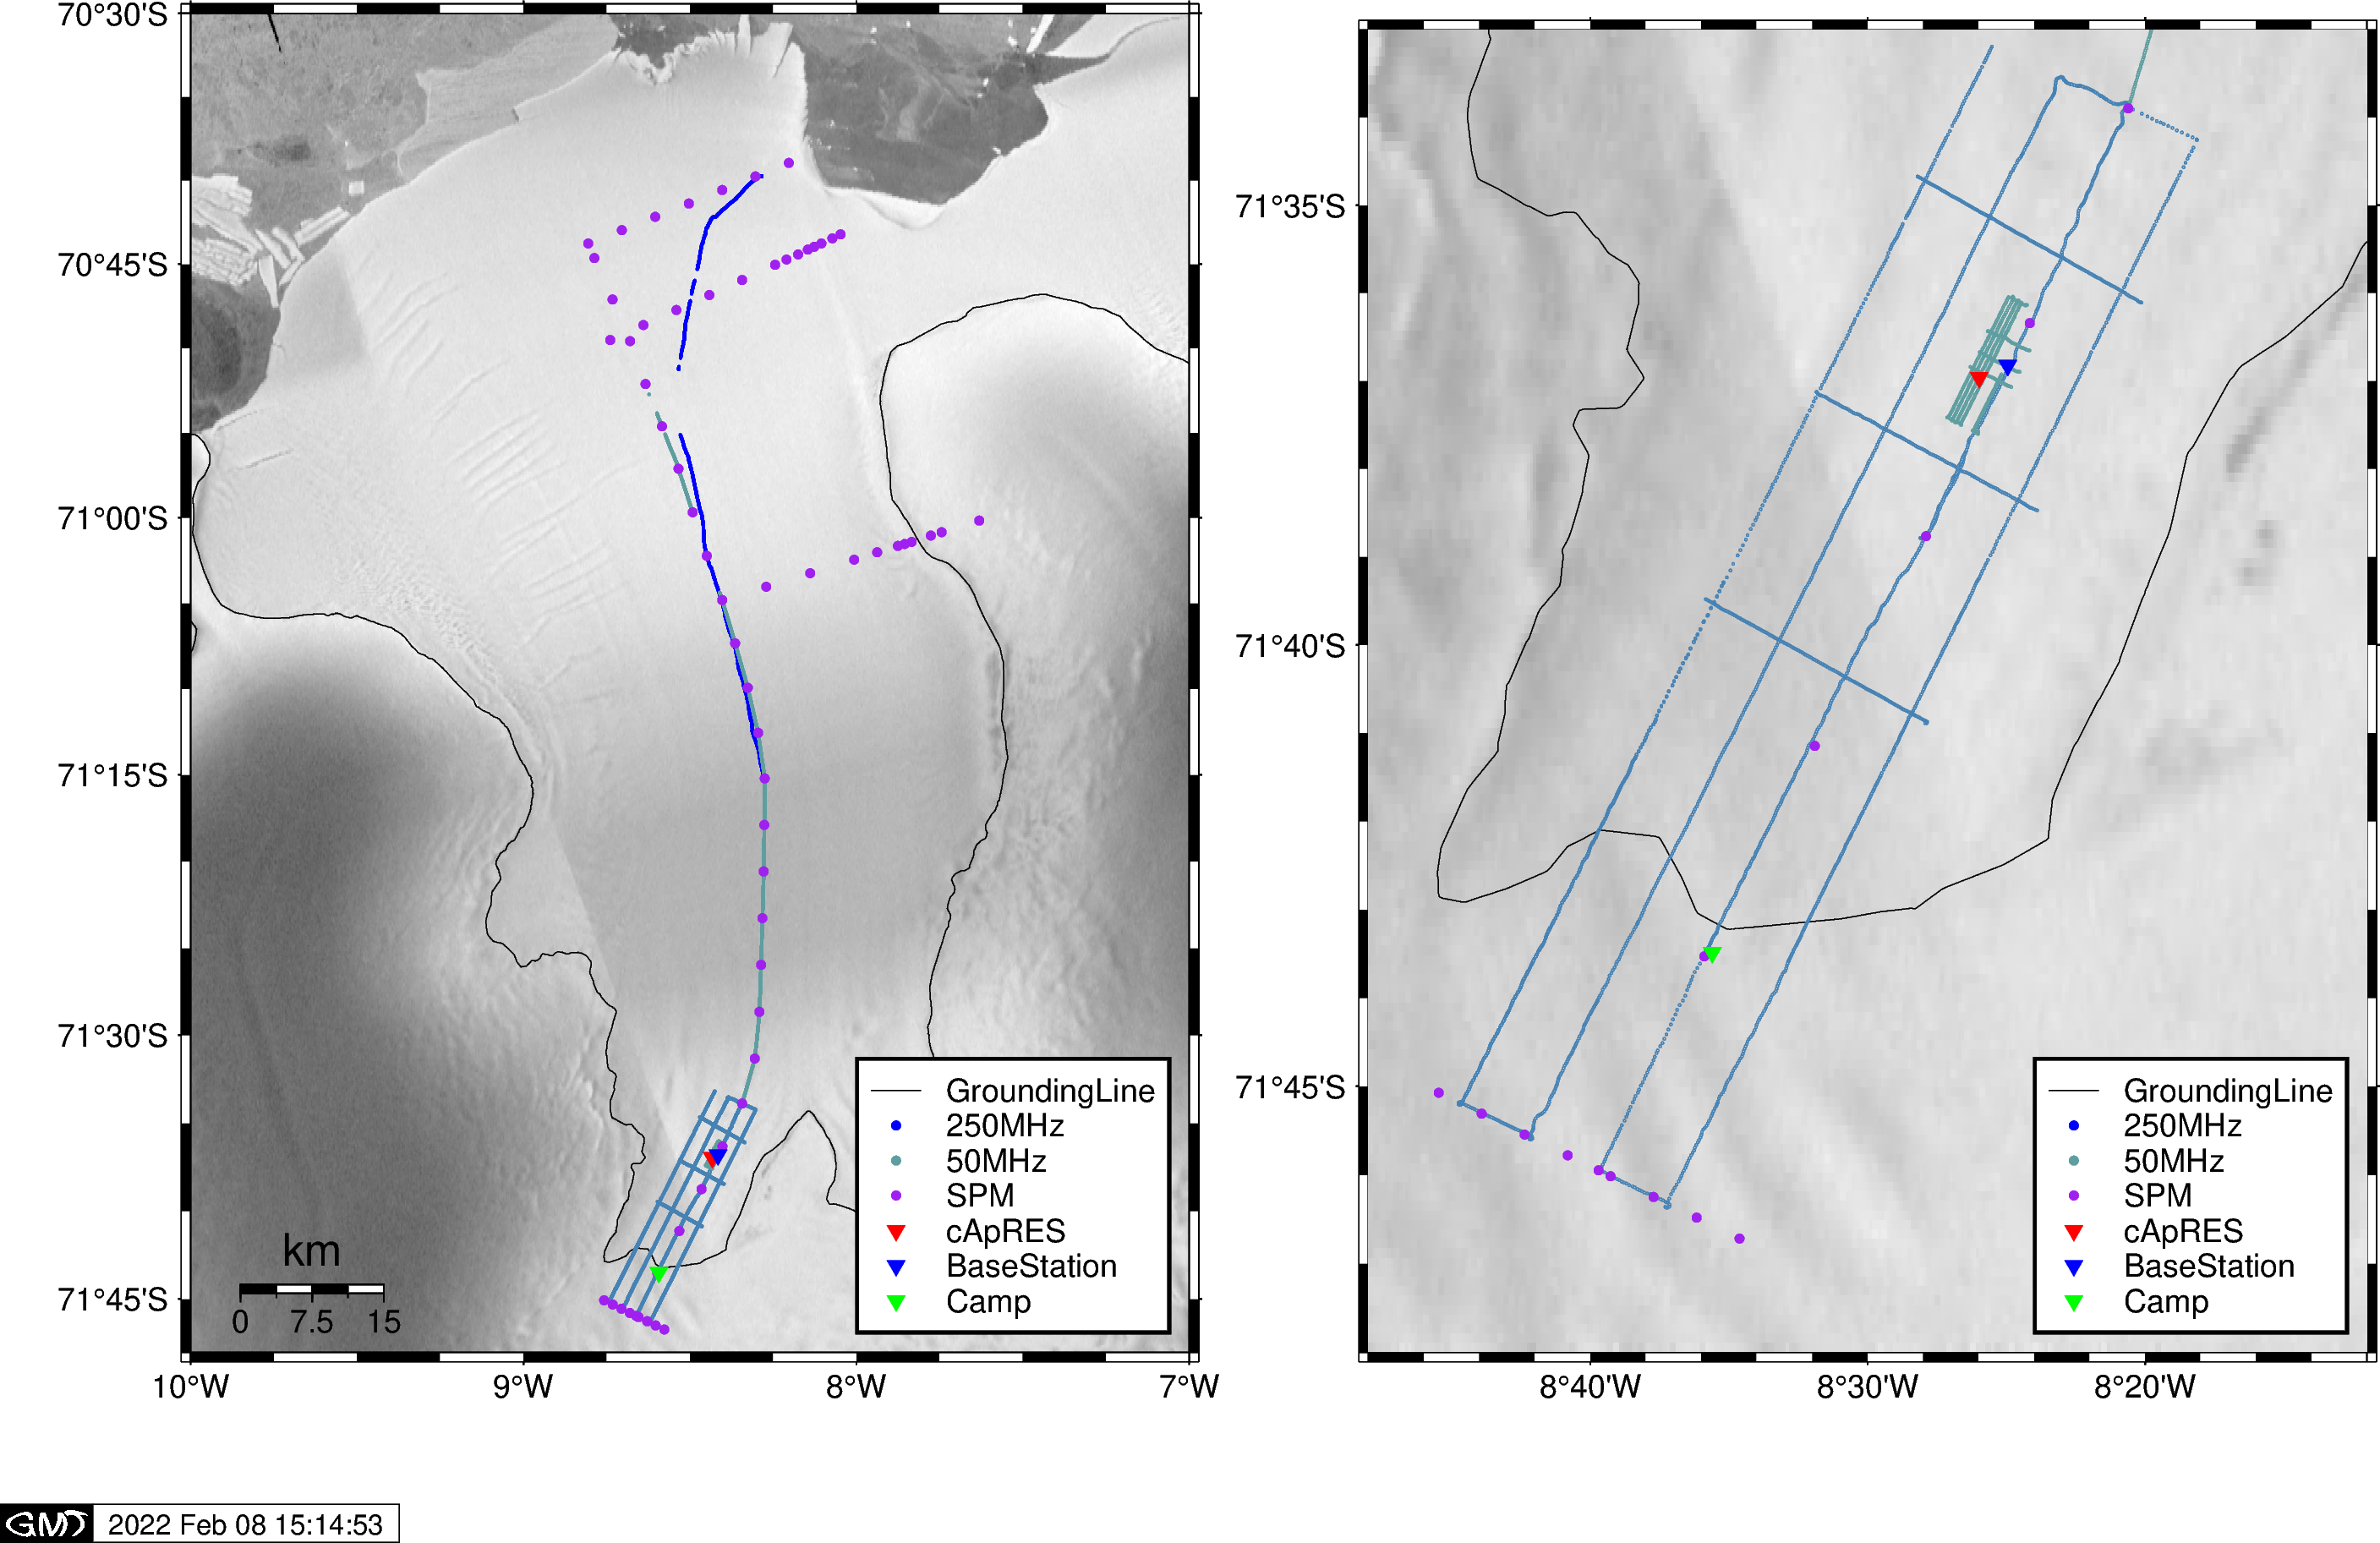
\includegraphics[width=\linewidth]{Figures/Overview.png}
  \caption{(Left) Larger-scale bird's eyes perspective of 250 MHz GPR, 50 MHz GPR, static \& polarimetric (SPM) and continuous ApRES (cApRES) locations at Ekström Ice Shelf, East Antarctica. (Right) Close-up of the survey grid close to the grounding-zone.}
  \label{fig:overview}
\end{figure}
ReMeltRadar's scientific focus (1) to understand \& quantify processes that govern ocean-induced melting at the base of ice shelves, and (2) to provide observational constraints on the spatial variability of ice rheology impacting ice-shelf buttressing strength. The area of interest is the Ekström Ice Shelf, East Antarctica, using the Neuyamer III station as a logistical hub for field surveys on the ice shelf and in the grounding zone. The first field season took place from November 2021 to January 2022. This report details the data collected and will serve as a baseline for envisaged repeat measurements in 2022/23. 

\pagebreak
\subsection{Team composition and chronology of data collection}
\begin{table}
\rowcolors{2}{gray!25}{white}
\begin{tabular}{llll}
  \rowcolor{gray!50}
  Name & Project& Deployment& Responsibility\\
  \hline
  Inka Koch (UT) & ReMeltRadar & 27.12.21-13.12.22& PulseEkko GPR\\
  Jonathan Hawkins (UCL) & ReMeltRadar  &27.12.21-13.12.22& HF ApRES\\
  Reinhard Drews (UT) & ReMeltRadar  &27.12.21-13.12.22& Science Coordination\\
  Reza Ershadi (UT) & ReMeltRadar &05.11.21-13.12.22& Rover, SPM\\
  Olaf Eisen (AWI) & ReMeltRadar  &05.11.21-13.12.22& Traverse Leader\\
  \hline
\end{tabular}
\caption{\label{TableGPR}Team composition of ReMeltRadar with members of University of Tübingen (UT), University College London (UCL), and Alfred Wegener Institute (AWI).}
\end{table}
\begin{table}
  \rowcolors{2}{gray!25}{white}
  \begin{tabular}{m{1.5cm} m{2.25cm} m{7cm} m{3cm}}
    \rowcolor{gray!50}
    Date & Frequency & Profile & File-ID\\
    \hline
    28.12.21 & 50, 100 MHz & Test profiles near NM& \textit{PE files}\\
    29.12.21 & 100 MHz & MPA01-MPA03, SPX4-SPX2 near NM& \textit{PE files}\\
    01.01.22 & 250 MHz  & NM-SPMA25 during traverse& \textit{PE files}\\
    02.01.22 & 50 MHz & GZ profiling along flow (SPMA25-SPMA21-GLPE3n-GLPE4s)& \textit{PE files}\\
    03.01.22 & 50 MHz & GZ profiling along flow (GLPE4s-GLPE1s-GLPE2n transfer to SPMA25)& \textit{PE files}\\
    04.01.22 & 50 MHz & GZ profiling along flow (GLPE7n-GLPE8s-GLPE5s)& \textit{PE files}\\
    05.01.22 & 50 MHz & GZ profiling across flow (XX points XX)& \textit{PE files}\\
    06.01.22 & 50 MHz & Finegrid along flow (XX points XX)& \textit{PE files}\\
    09.01.22 & 50 MHz & Finegrid across flow (XX points XX)& \textit{PE files}\\
    10.01.22 & 50 MHz & Along-flow Camp-NM (SPMA21-SPMA10)& \textit{PE files}\\
    12.01.22 & 50 MHz & Camp-NM continuation (SPMA10 - XX)& \textit{PE files}\\
    \hline
  \end{tabular}
  \caption{\label{TableGPR}Overview of GPR measurements taken with the PulseEkko radar from Sensors\&Software. Details for the system setup and individual profiles are found in Section \ref{SecGpr}. Operator: I. Koch.}
Here we need a table such as table \label{TableGPR} for each sensor. 
\end{table}

\pagebreak
\section{Data structure and initial source codes}
\textbf{RD, JH}

\pagebreak
\section{GPR: Data example, field picture, system setup and profile specifics}
\label{SecGpr}
\textbf{IK}
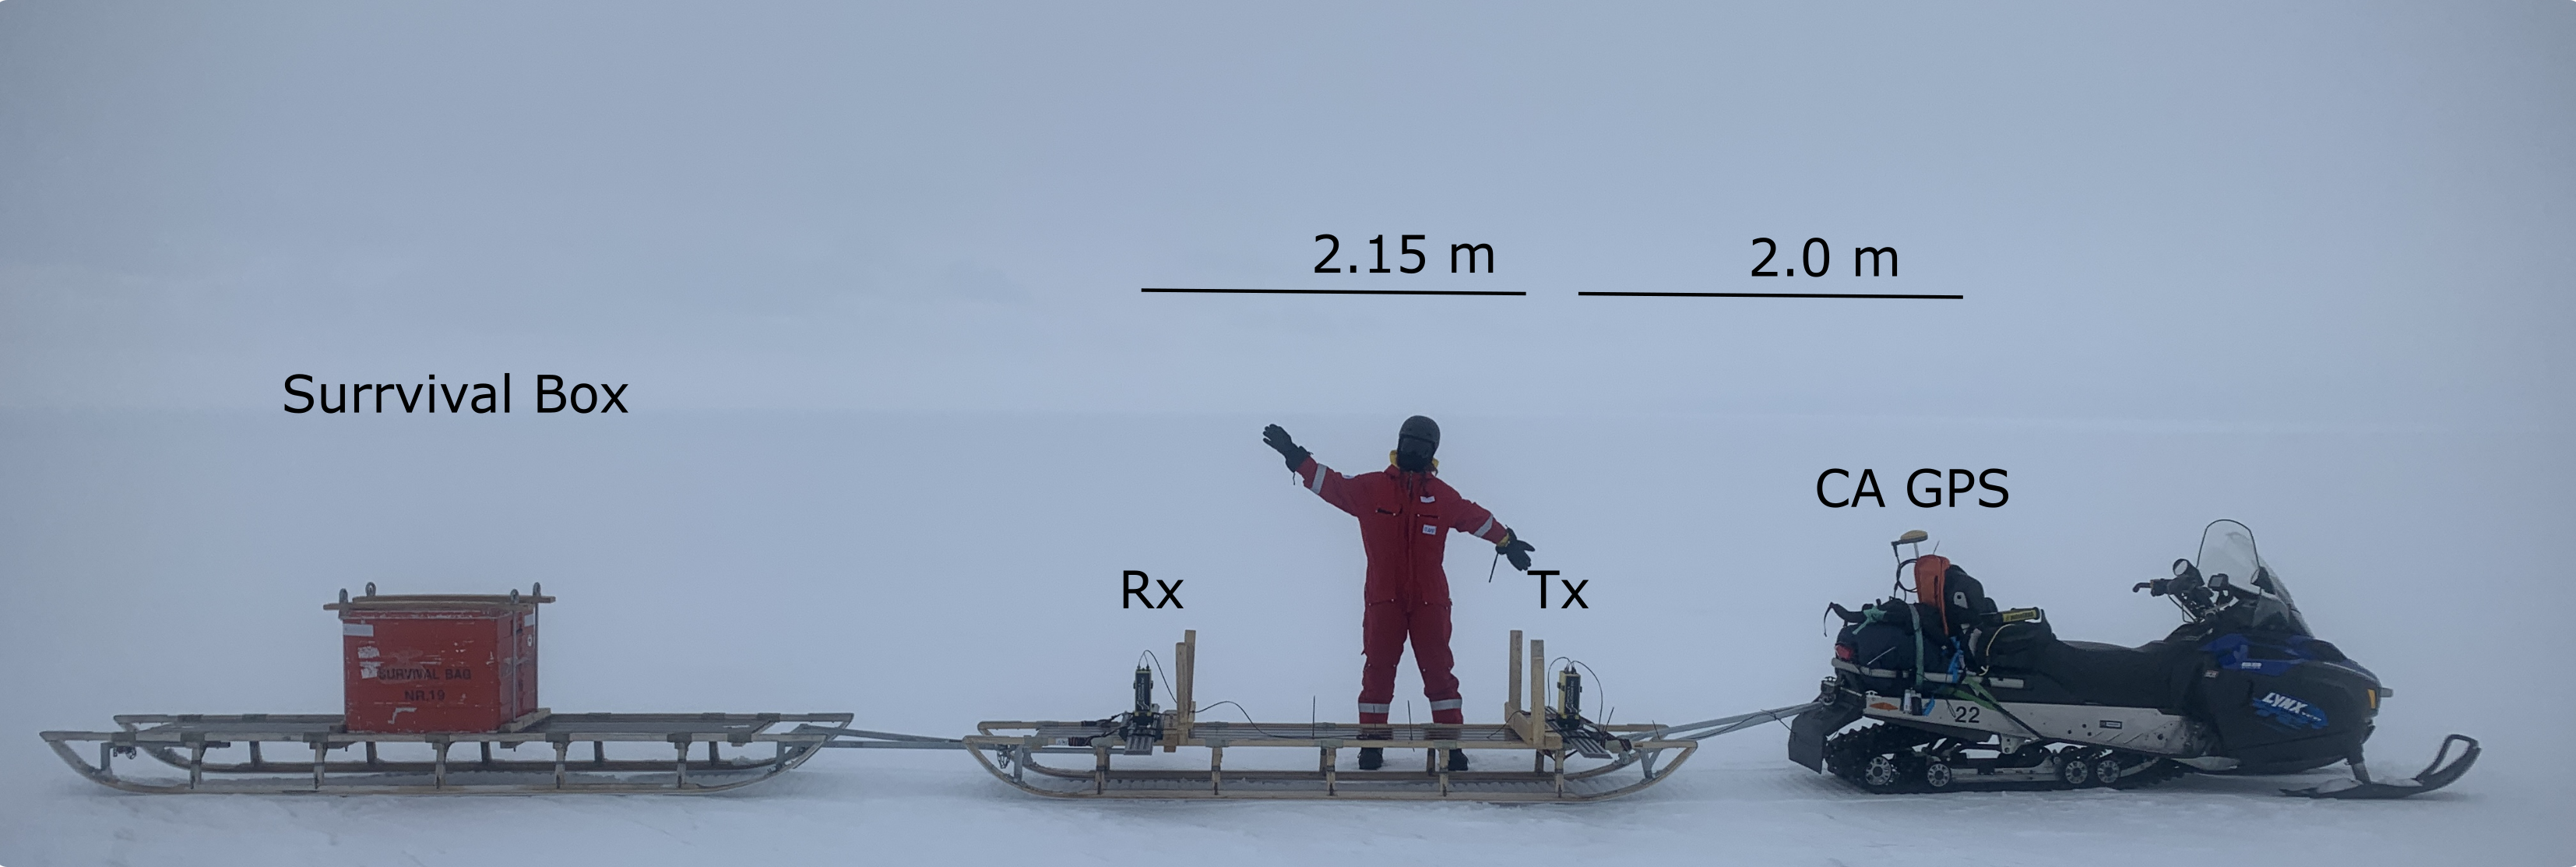
\includegraphics[width=\textwidth]{Figures/PulseEkko/RadarSetup.png}

\pagebreak
\section{SPM: Data example, field picture, system setup and site specifics}
\textbf{RE}
\label{SecSPM}

\pagebreak
\section{HF ApRES: Data example, field picture, system setup and profile specifics}
\label{SecHFApRES}
\textbf{JH}

\pagebreak
\section{cApRES: Data example, field picture, system setup and site specifics}
\label{SeccApRES}
\textbf{RE,JH}

\pagebreak
\section{Rover-ApRES: Data example, field picture, system setup and site specifics}
\label{SecRoverApRES}
\textbf{RE}

%\ProtocolTable{Setup PulseEkko Radar}{N/A}{PulseEkko 50 MHz}{N/A}{I. Koch}{N/A}

% \begin{minipage}[t]{\textwidth}
%
% \end{minipage}



\end{document}